\documentclass[11pt,fleqn]{article}
\usepackage{../cs188,latexsym,epsf, amsmath,amsfonts,graphicx,url}
\lecture{8}
\def\title{Note \the\lecturenumber}
\begin{document}
\maketitle


\iffalse
\documentclass[11pt,fleqn]{article}
\usepackage{latexsym,epsf,amsmath,amsfonts,graphicx,url}

\title{Note 8}

\newcommand{\F}{\mathbb{F}}
\newcommand{\Z}{\mathbb{Z}}
\newcommand{\Q}{\mathbb{Q}}
\newcommand{\R}{\mathbb{R}}
\newcommand{\C}{\mathbb{C}}

\begin{document}

\maketitle
\fi


We have developed our techniques for probabilistic reasoning in the context of \textit{static} world, in which each random variable takes a single fixed value. For example, when probing the cavity, we assume that whatever tooth has a cavity remains cavitary during the process of probing; when forecasting the weather, we assume that whether the forecaster says a rainy day or not the weather does not change in that day. In many real-world problems, we want to reason about a sequence of observations. As a follow-up of the previous weather example, consider the task of monitoring every day's actual weather based on the historical weather forecasts. Unlike the previous example, here the \textit{dynamic} aspects of the problem are essential since the weather changes day by day. Other examples include robot localization where robot moves in a space and we want to know the robot's current location based on a sequence of range sensor observations, speech recognition where the task is to figure out the actual words people say based on a segment of rapidly changing acoustic signals, etc. 

\section{Markov Model}
Markov chain (MC) is a common model to capture the dynamics of the problem. MC can be considered as a special Bayes' net where each node corresponds to the state in a given time step.

\begin{center}	
	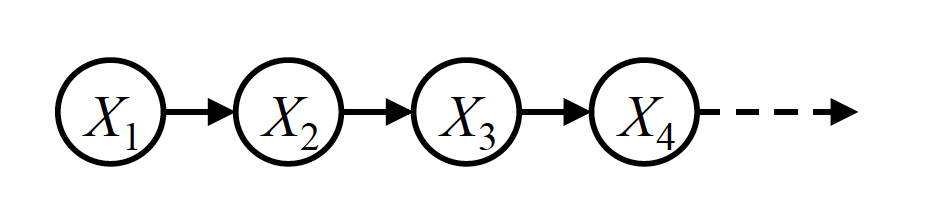
\includegraphics[width=10cm]{img/mc}
\end{center} 

MC makes the assumption that the state at each time step depends only on the previous state. In other words, given the current state $X_t$, the future state $X_{t+1}$ is conditionally independent of the entire past states $X_{t-1},\cdots,X_1$,
\begin{align}
P(X_{t+1}|X_1,\cdots,X_t) = P(X_{t+1}|X_t)
\end{align}
$P(X_{t+1}|X_t)$ is called transition model or transition probability in the MC. Another assumption that we will make on the MC throughout the course is the \textit{stationary} assumption, which states that the transition probability does not change over time, i.e.,
\begin{align}
P(X_{t+1}|X_t) = P(X_t|X_{t-1}) = \cdots
\end{align}
To fully characterize the MC, we only need a CPT for the transition model and a CPT for the probability distribution of the initial state $P(X_1)$. Once we have these two CPTs, we can represent the joint probability distribution of all states in the MC and can perform various kinds of inference tasks thereafter. 

There is a inference task that is of particular interest in the MC - the probability distribution of the state at a given time step, i.e., $P(X_t)$. For example, $X_t$ is the weather (rain/sun) in day $t$. $P(X_t)$ is the chances of the weather being rainy and sunny, respectively. By simply using the probability law on marginalization and chain rule, we can derive an iterative algorithm to calculate $P(X_t)$ as follows,
\begin{align}
\label{eqn:mini_forward}
P(x_t)&= \sum_{x_{t-1}}P(x_t,x_{t-1})\nonumber\\
&= \sum_{x_{t-1}} P(x_t|x_{t-1})P(x_{t-1})
\end{align}
Since we know the probability distribution of the initial state $P(x_1)$ and transition model $P(x_t|x_{t-1})$, we can solve $P(x_t)$ for $t=2,3,\cdots$ using (\ref{eqn:mini_forward}). This iterative procedure is called Mini-Forward algorithm.

A interesting phenomenon regarding $P(X_t)$ for a stationary MC is that as $t$ goes to infinity, $P(X_t)$ converges to a fixed probability distribution (you can think of it as a fixed probability table) whatever probability distribution the initial state has. To derive what distribution $P(X_t)$ converges to, we can use Mini-Forward algorithm,
\begin{align}
\label{eqn:stat_dist}
P(x_{\infty})=P(x_{\infty+1}) &= \sum_{x_{\infty}}P(x_{\infty+1},x_{\infty})\nonumber\\
&= \sum_{x_{\infty}} \underbrace{P(x_{\infty+1}|x_{\infty})}_{\text{transition probability}}P(x_{\infty})
\end{align}
In addition, we know that the probability should be summed up to one, i.e.,
\begin{align}
\label{eqn:one}
\sum_{x_\infty} P(x_\infty)=1
\end{align}
Note that (\ref{eqn:stat_dist}) and (\ref{eqn:one}) provide a system of linear equations with respect to $P(x_\infty)$. Treating the convergence distribution $P(x_\infty)$ as unknown variables, we can solve it from (\ref{eqn:stat_dist}) and (\ref{eqn:one}). $P(x_\infty)$ is called stationary distribution of the MC, and (\ref{eqn:stat_dist}) and (\ref{eqn:one}) give a bunch of conditions that the stationary distribution should satisfy.


\section{Hidden Markov Model}
As aforementioned, in many real-world problems we cannot directly gather evidence on the exact state but some noisy observations related to the actual state. Say, in the robot localization problem, we can only observe a sequence of noisy range sensor readings and hope to infer the actual location of the robot based on the sensor measurements. In this problem, the actual robot location is the hidden state variable (something we would like to know but not observable), the sensor measurements are evidence/observation variables (something we can directly observe). The model for this kind of problem is hidden Markov model.

Hidden Markov model (HMM) (shown below) consists of state variables $X_t$ that evolve according to Markov property and observable evidence variables $E_t$. An HMM is defined by initial state distribution $P(X_1)$, transition model $P(X_{t+1}|X_t)$ and emission model $P(E_t|X_t)$. 

\begin{center}	
\label{fig:hmm}
	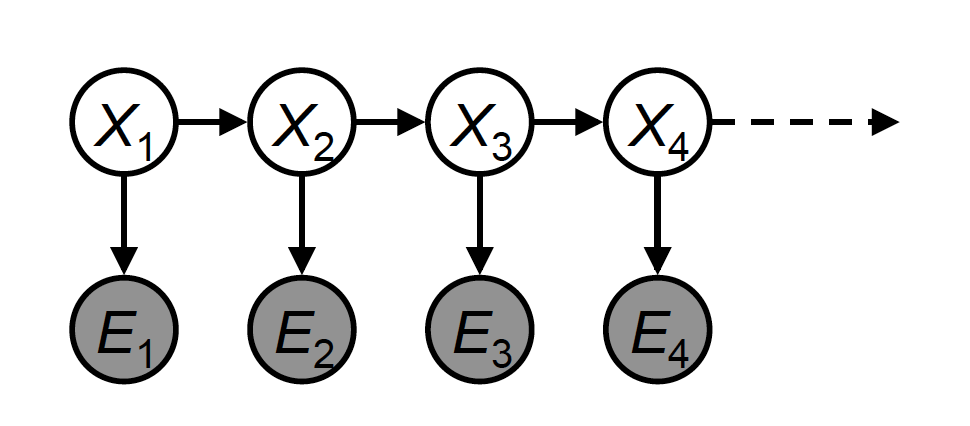
\includegraphics[width=10cm]{img/hmc}
\end{center}

Just like MC, HMM is another special type of Bayes net that is fully characterized by the three CPTs, i.e., initial distribution, transition and emissions. In the ghostbuster example we've seen in the class, the initial distribution is uniform, the transition model assigns high probability to move clockwise and some small probability to move in a random direction, and emission model gives the probability of a coordinate being red or green. There are two important conditional independence assumptions encoded in an HMM:
\begin{itemize}
\item Given the current state $X_t$, future state $X_{t+1}$ is conditionally independent of all past states $X_t,\cdots,X_1$ and past evidences $E_t,\cdots,E_1$.

\item Given the current state $X_t$, current evidence $E_t$ is independent of every other variable in the HMM
\end{itemize}

With the problem being formulated as an HMM, we can then perform some inference tasks. The first inference task we are interested in is \textit{filtering/monitoring}, which is to find the distribution of the current state given the evidences collected up to now, i.e., $P(X_t|e_1,\cdots,e_t)$. We call this conditional probability the belief state, which is often denoted as $B_t(X)$.

Although we could apply various techniques learned from the Bayes' net lecture, such as variable enumeration and variable elimination, to compute this particular query, we 
would like to have a recursive algorithm that maintains a current belief and updates the belief at each time step. The forward algorithm is such an algorithm, which computes the new belief based on the current belief and new evidence. It can be derived as follows:
\begin{align}
\label{eqn:def_cond}
B_{t+1}(X) = P(X_{t+1}|e_1,\cdots,e_{t+1})&=\frac{P(X_{t+1},e_{t+1}|e_1,\cdots,e_{t})}{P(e_{t+1}|e_1,\cdots,e_{t})}\\
\label{eqn:prop}
&\propto P(X_{t+1},e_{t+1}|e_1,\cdots,e_{t})\\
\label{eqn:prob_law}
&=\sum_{x_{t}} P(X_{t+1},x_{t},e_{t+1}|e_1,\cdots,e_{t})\\
\label{eqn:chain_rule}
&=\sum_{x_{t}} P(e_{t+1}|X_{t+1},x_{t},e_1,\cdots,e_{t})P(X_{t+1}|x_{t},e_1,\cdots,e_{t})P(x_{t}|e_1,\cdots,e_{t})\\
\label{eqn:cond_indep}
&=P(e_{t+1}|X_{t+1})\sum_{x_{t}}P(X_{t+1}|x_{t})P(x_{t}|e_1,\cdots,e_{t})\\
\label{eqn:def_prev_belief}
&=P(e_{t+1}|X_{t+1})\sum_{x_{t}}P(X_{t+1}|x_{t})B_{t}(X)
\end{align}
(\ref{eqn:def_cond}) is by the definition of conditional probability; (\ref{eqn:prop}) states that $P(X_{t+1}|e_1,\cdots,e_{t+1})$ is proportional to $P(X_{t+1},e_{t+1}|e_1,\cdots,e_{t})$, so once we get $P(X_{t+1},e_{t+1}|e_1,\cdots,e_{t})$ we can compute $P(X_{t+1}|e_1,\cdots,e_{t+1})$ by renormalizing the entries in $P(X_{t+1},e_{t+1}|e_1,\cdots,e_{t})$; In (\ref{eqn:prob_law}) we add $X_{t}$ into the probability distribution, and this is because we want to derive the future belief in terms of conditional probabilities of the current state $X_t$; (\ref{eqn:chain_rule}) expands $P(X_{t+1},x_{t},e_{t+1}|e_1,\cdots,e_{t})$ via chain rule; (\ref{eqn:cond_indep}) simplifies the conditional probability terms using the conditional independence assumptions encoded in the HMM - $P(e_{t+1}|X_{t+1},x_{t},e_1,\cdots,e_{t})=P(e_{t+1}|X_{t+1})$ and $P(X_{t+1}|x_{t},e_1,\cdots,e_{t})=P(X_{t+1}|x_t)$.

The second inference task of particular interest is to find the \textit{most likely explanation} (MLE) that generates the given observations, which in mathematical language is to compute 
\begin{align}
arg\max_{x_1,\cdots,x_t} P(x_1,\cdots,x_t|e_1,\cdots,e_t)
\end{align}

A brute force algorithm to find MLE is to enumerate all possible state sequence and select the one that maximizes $P(x_1,\cdots,x_t|e_1,\cdots,e_t)$. But this algorithm is quite slow. Assume that each hidden node can take two state values, then there are $2^t$ state sequences to pick from. In contrast, Viterbi is a linear-time algorithm based upon dynamic programming.

Viterbi algorithm keeps track of a message $m_{t+1}[x_{t+1}]=\max_{x_1,\cdots,x_t} P(x_1,\cdots,x_t,x_{t+1},e_1,\cdots,e_t)$ and update the message in the following iterative way:
\begin{align}
m_{t+1}[x_{t+1}]&=\max_{x_1,\cdots,x_t} P(x_1,\cdots,x_t,x_{t+1},e_1,\cdots,e_{t+1})\\
&=\max_{x_1,\cdots,x_t}P(e_{t+1}|e_1,\cdots,e_t,x_1,\cdots,x_{t+1})P(x_{t+1}|e_1,\cdots,e_t,x_1,\cdots,x_t)P(x_1,\cdots,x_t,e_1,\cdots,e_t)\\
&=P(e_{t+1}|x_{t+1})\max_{x_1,\cdots,x_t}P(x_{t+1}|x_t)P(x_1,\cdots,x_t,e_1,\cdots,e_t)\\
&=P(e_{t+1}|x_{t+1})\max_{x_t}P(x_{t+1}|x_t)\max_{x_1,\cdots,x_{t-1}}P(x_1,\cdots,x_t,e_1,\cdots,e_t)\\
&=P(e_{t+1}|x_{t+1})\max_{x_t}P(x_{t+1}|x_t)m_t[x_t]
\end{align}
Note that $m_2[x_2] = \max_{x_1} P(x_1,x_2,e_1,e_2) = \max_{x_1} P(e_2|x_2)P(e_1|x_1)P(x_2|x_1)P(x_1)$ is easy to compute from the probability distribution of the initial state $X_1$, transition model and emission model. Once we get $m_2[x_2]$, we can compute $m_3[x_3],\cdots,m_t[x_t]$ using the above iterative update equation. The MLE is just $x_1,\cdots,x_t$ that maximize $m_1[x_1],\cdots,m_t[x_t]$, respectively.

Note that the update in the Viterbi algorithm looks exactly the same as the forward algorithm except that the summation is changed to the max operator.

\section{Particle Filtering}
In this section we consider an algorithm that finds an approximate solution for the filtering task, i.e., $P(X_t|e_1,\cdots,e_t)$. This is in contrast to forward algorithm, which compute the exact value of $P(X_t|e_1,\cdots,e_t)$. Firstly, why do we even need approximate inference? We can find from the previous contents that in order to perform forward algorithm, we need a way to represent transition model, emission model as well as the belief state that is generated along the way. This can be done trivially if the state is discrete, since we can always use probability tables to represent those. However, when the state is continuous it becomes hard to represent transition and emission model and to keep track of belief states. In the case where the problem has a very large space, you may need excessive memory to store those probability tables. We would like an efficient method to perform filtering task irrespective of the size of state space or even a continuous state space. Particle filtering is an approximate solution to find the belief state $P(X_t|e_1,\cdots,e_t)$, which approximates the belief states by a set of samples/particles.

At time $t$, we start with a set of particles representing the old belief state $P(X_{t-1}|e_1,\cdots,e_{t-1})$. Then the particle filtering takes the following three steps to update the belief: 

1. Elapse time: each particle is moved by sampling it next position from the transition model. For instance, we sample the next position of the green particle located at $(3,3)$ from the transition probability $P((x',y')|(3,3))$, which turns out to be $(3,2)$. So we move the particle at $(3,3)$ to $(3,2)$. We sample the next positions for all particles on the map and move them accordingly.

2. Weighting: each particle is assigned with a weight which equals to $P(e_t|x_t)$ - the likelihood of generating the newly observed evidence $e_t$.

3. Resampling: we create a new set of particles by sampling the existing set of particles. The chance of a particle being sampled is equal to its weight.

The new set of particles represents the new belief state $P(X_t|e_1,\cdots,e_t)$. We can approximate  $P(X_t=x_t|e_1,\cdots,e_t)$ by counting the number of particles at $x_t$ and divided by the total number of particles.


\begin{center}	
	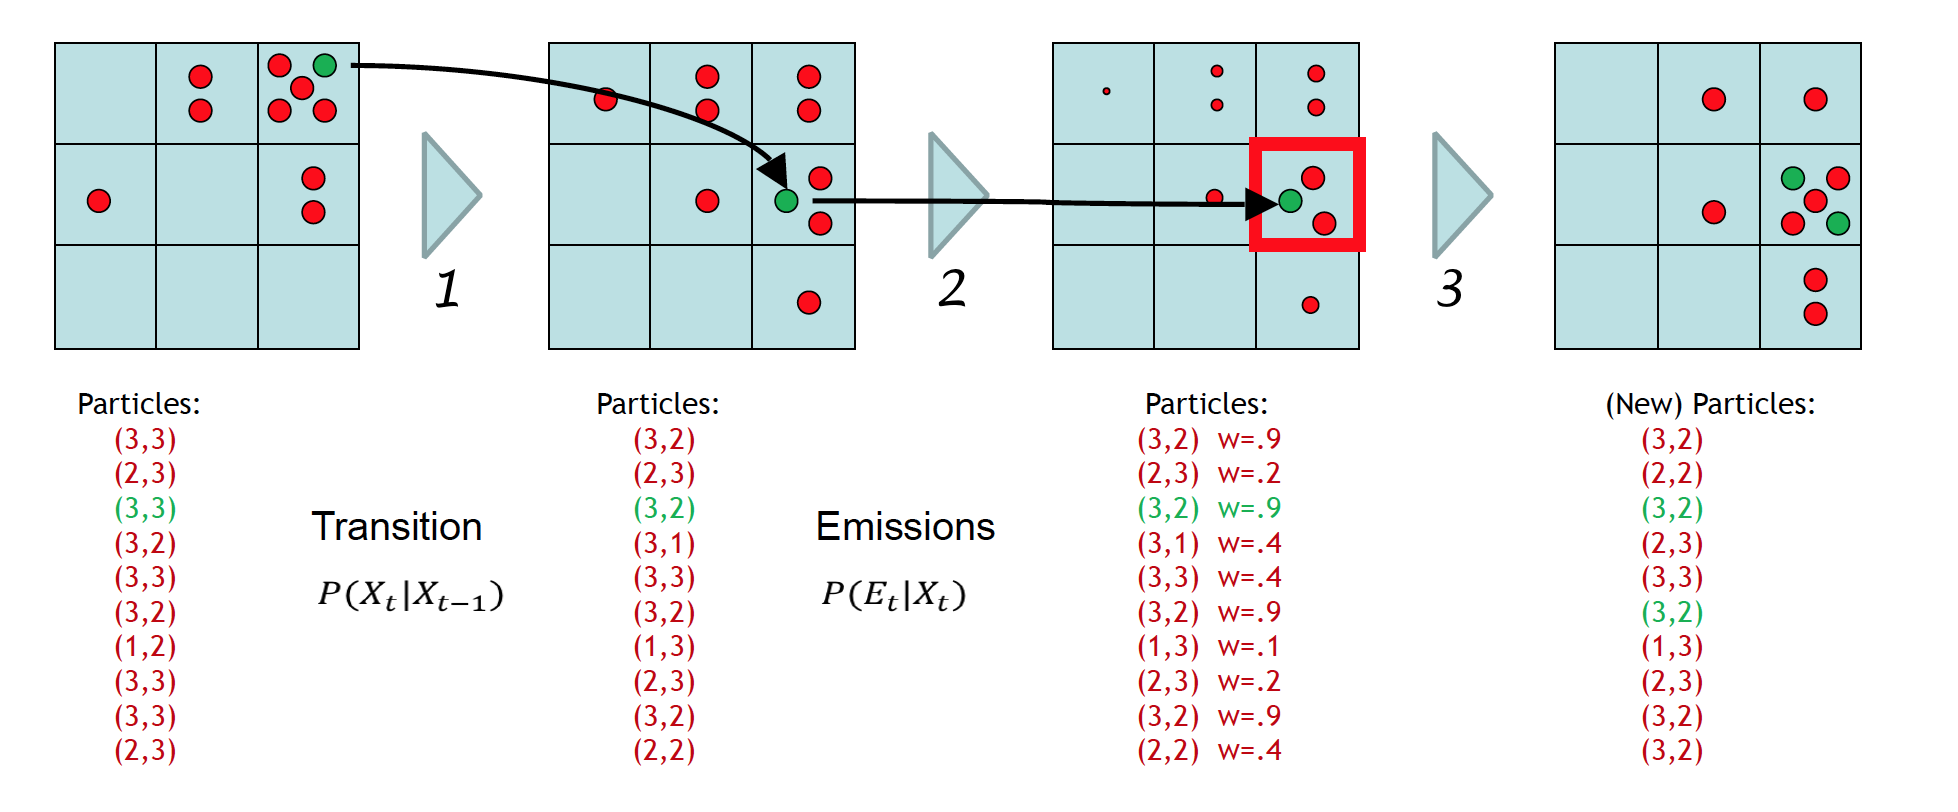
\includegraphics[width=15cm]{img/pf}
\end{center} 






\end{document}
